%\section{Implementation}
This chapter is dedicated to the implementation of the presented system. In this chapter we will explain in detail what has been implemented and how. 

\section{System}
%%In this section we will elaborate on the implementation for this project. We will delve into the system that the project is running on. We will shortly discuss the technological choices we have made and explain our reasons so.
%%%% Rasmus: Needs to be rewritten. Stupid. What do we want here?
The system has been implemented using Java and Servlets for the backend, and JSP and Javascript for displaying the webpages. We have chosen to use MySQL as a database since it is known to all the members. The database is used to store the policies. 
\\The frontend and backend have been developed to work together as much as possible and the backend to provide all the information necessary for the frontend. However, because we have chosen to serialize the policies to JSON, in the frontend these JSON have to be deserialised and parsed. 
The core part of the system is represented by the servlet that runs the whole application. Inside this servlet there is a timer so policies are executed at a specific interval. The servlet manages all the requests from the frontend and takes appropriate action. 
\subsection{Interfaces}
There are two interfaces that describe the methods of Statements and Value classes. Each statement should implement an execute method, in which specific execution is done. 
\subsection{Domain}
\begin{figure}
	\centering
    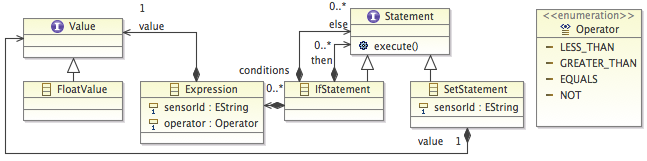
\includegraphics[scale=0.55]{chapters/implementation-model-expression-language.png} 
	\caption{The core classes in the \textit{expression language}.}
	\label{fig:ecore-sensors-actuators}
\end{figure}

A statement can either be a SetStatement or an IfStatement. The SetStatement sets an value in the simulator (in effect it is an actuator). It is possible to have nested IfStatements, making the policies both flexible and simple. An IfStatement can contain multiple expressions that all are being anded when evaluated. If the user wants to make an IfStatement with or between the expressions, will have to use a nested IF. The optimal solution to this would be to make a safe left-recursive model. We did not have enough time for this, but we will elaborate further on this subject in the \nameref{chapter:discussion} section. 

An Expression has three variables, the sensorId, the operator and a value of type Value. When the policy engine is running, each expression is being evaluated. The current value of the sensor is fetched and compared to the desired value using the operator. An expression can contain the following operators; <, >, <=, >=, !=,=. 
If the evaluation of the expression is true, then the statement is executed.

The FloatValue class implements the Value interface and it represents a value of type float. This is used to set the values of the sensors, as those can be of float type. However, because there is no possibility at the moment to set a float value using the REST interface of the simulator, this value is converted into an integer before sending it to the server.

A Policy object consists of statements and the policy can be run by executing those statements. A PolicyEntity object holds a policy and different properties of that policy such as name, description, interval, id and active. The interval property defines from which time to which time should the policy be enforced to run. This is implemented as a separate class, Interval, because of the serialization logics.  The active property represents the status of the policy as in if the user wishes for this policy to be executed (active) or not (not active).
\section{Persistence}
We have decided to have our policies stored in a database. The database chosen was MySQL as it is well known and used by all the members. Because we do not have a complex persistence system, we decided to use the simple JDBC for connecting and querying the database, and not use any frameworks. 
\\Methods for communicating with the database are defined in the DataAccessLayer class. There are the methods for creating, reading, updating and deleting policies. In addition, it is of great interest to have a method that returns only the policies that are running at the current time. 
\\Because the fact that different policies may operate on the same sensors, we decided to use a cache to store each sensor's value. This reduces the number of queries to the simulator server so it does not crash. This cache is implemented using a hashtable and stores the value of the sensor. After executing all the active policies at that moment, this cache is cleared. 
\section{Simulator querying}
To communicate with the simulator's server there is the Connection class for that. It provides methods for connecting to the server and parses the JSON received from it. There are several methods implemented that parse the response of the server and offer information such as - a list with the sensors in a room by providing the room id, a list with all the sensors of a certain type (e.g ac, light, heater etc.) The most two important methods are for retrieving the sensor's value and setting it to a specific one. 
%\section{Request Flow} Somebody added Request Flow? What should be here?? Nothing?